\section{Pipelining}
In pipelinging we overlap instructions in defferent stages
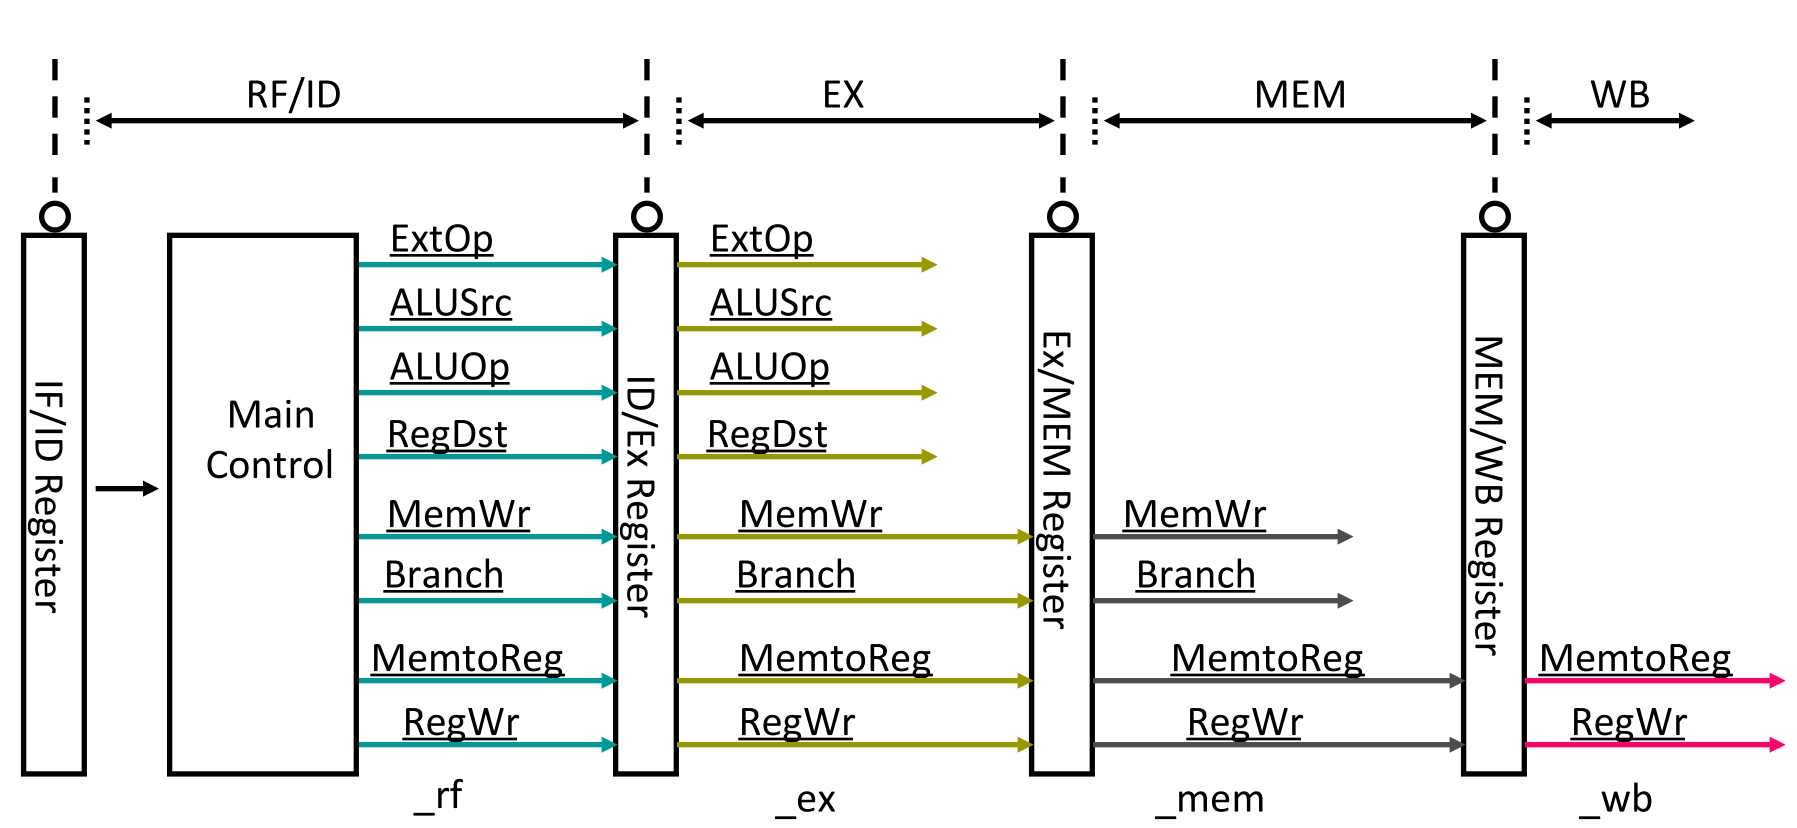
\includegraphics[width=\linewidth]{png/pipe.png}
There are hazards, these include \textbf{structural hazards}
where a required resource is busy, \textbf{data harzards} where we must wait previous
instructions to produce/consume data, and \textbf{control hazards} where next PC
depends on previous instruction.

\subsection*{Structural Hazards}
two instructions are trying to use the same hardware within the same cycle, to
solve this we can make all the instructions the same length

\subsection*{Data Dependencies}
Dependencies for instruction $j$ following instruction $i$
\begin{itemize}
\item Read after Write (RAW or true dependence)
	\par Instruction $j$ tries to read before instruction $i$ tries to write it
\item Write after Write (WAW or output dependence)
	\par Instruction $j$ tries to write an operand before $i$ writes its value
\item Write after Read (WAR or (anti dependence))
	\par Instruction $j$ tries to write a destination before it is read by $i$
\end{itemize}
\textbf{Solutions for RAW Hazards}: We can delay the reading of an instruction
until data is available, to do this we can insert pipeline bubbles, can also write
to the register file in the first half of a cycle and then read in the second half.

\textbf{Forwarding:} Another solution is forwarding or pushing the data to an
appropriate unit.

We can also reorder instructions to deal with RAW hazards
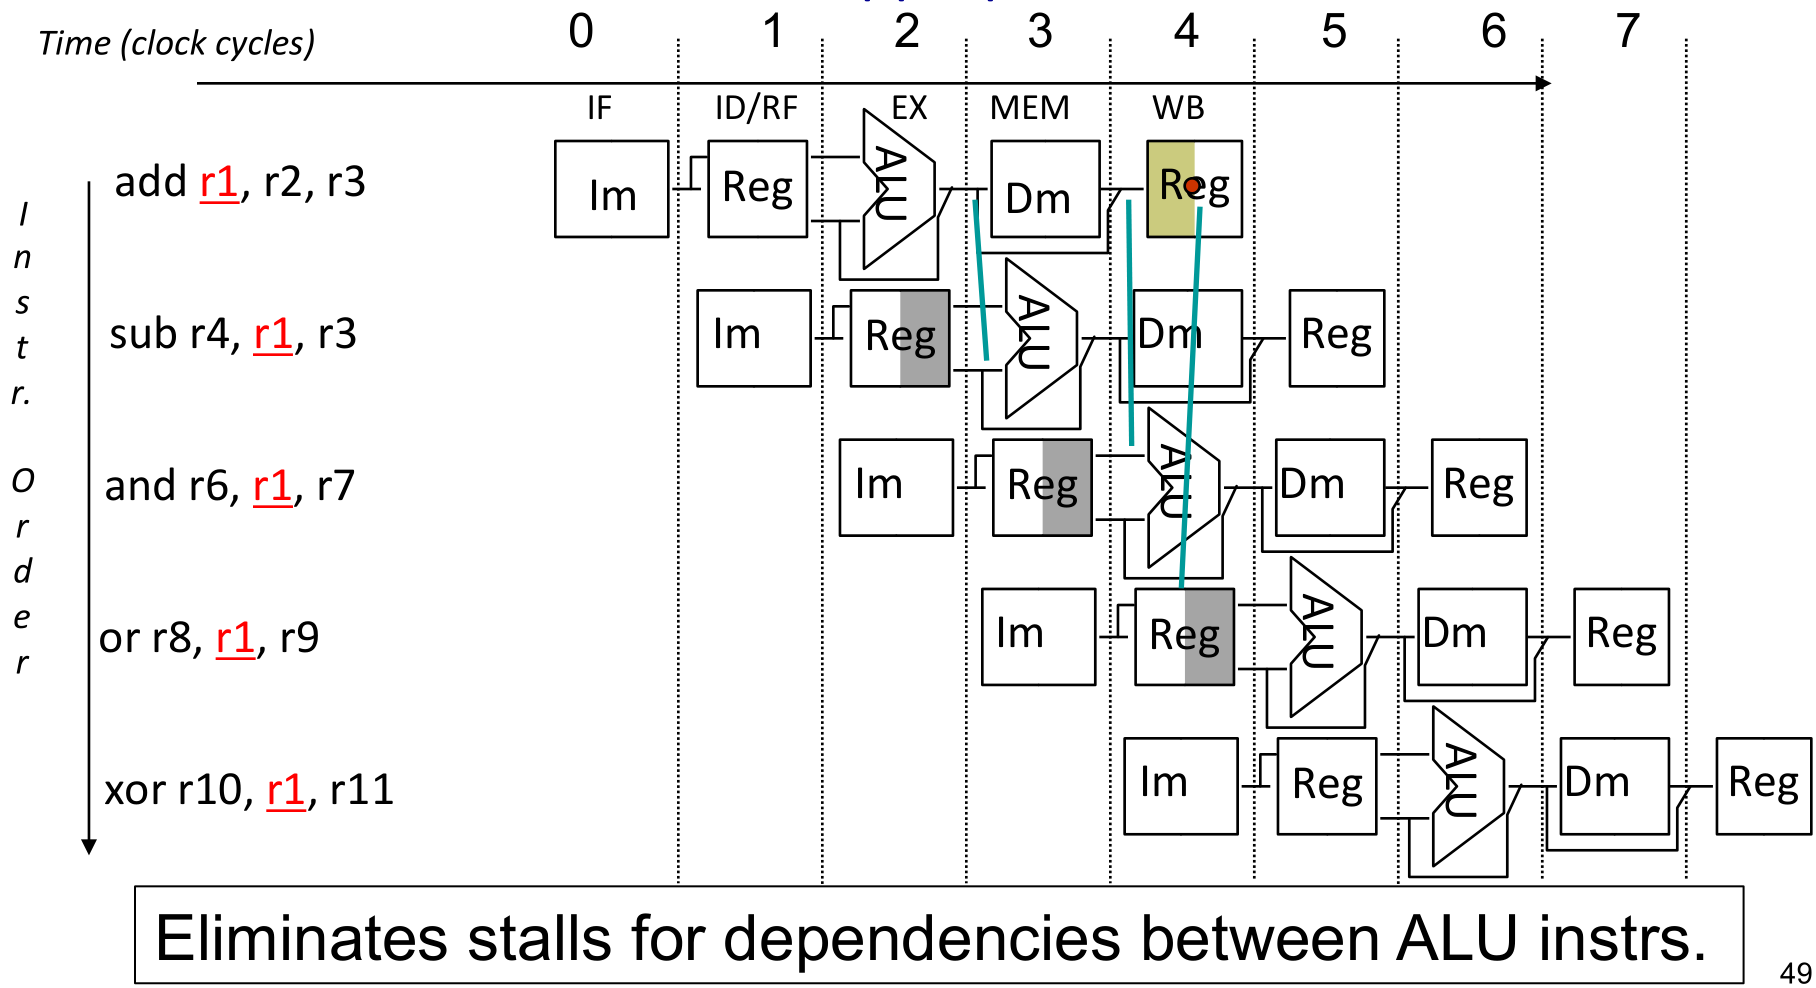
\includegraphics[width=\linewidth]{png/forwarding.png}
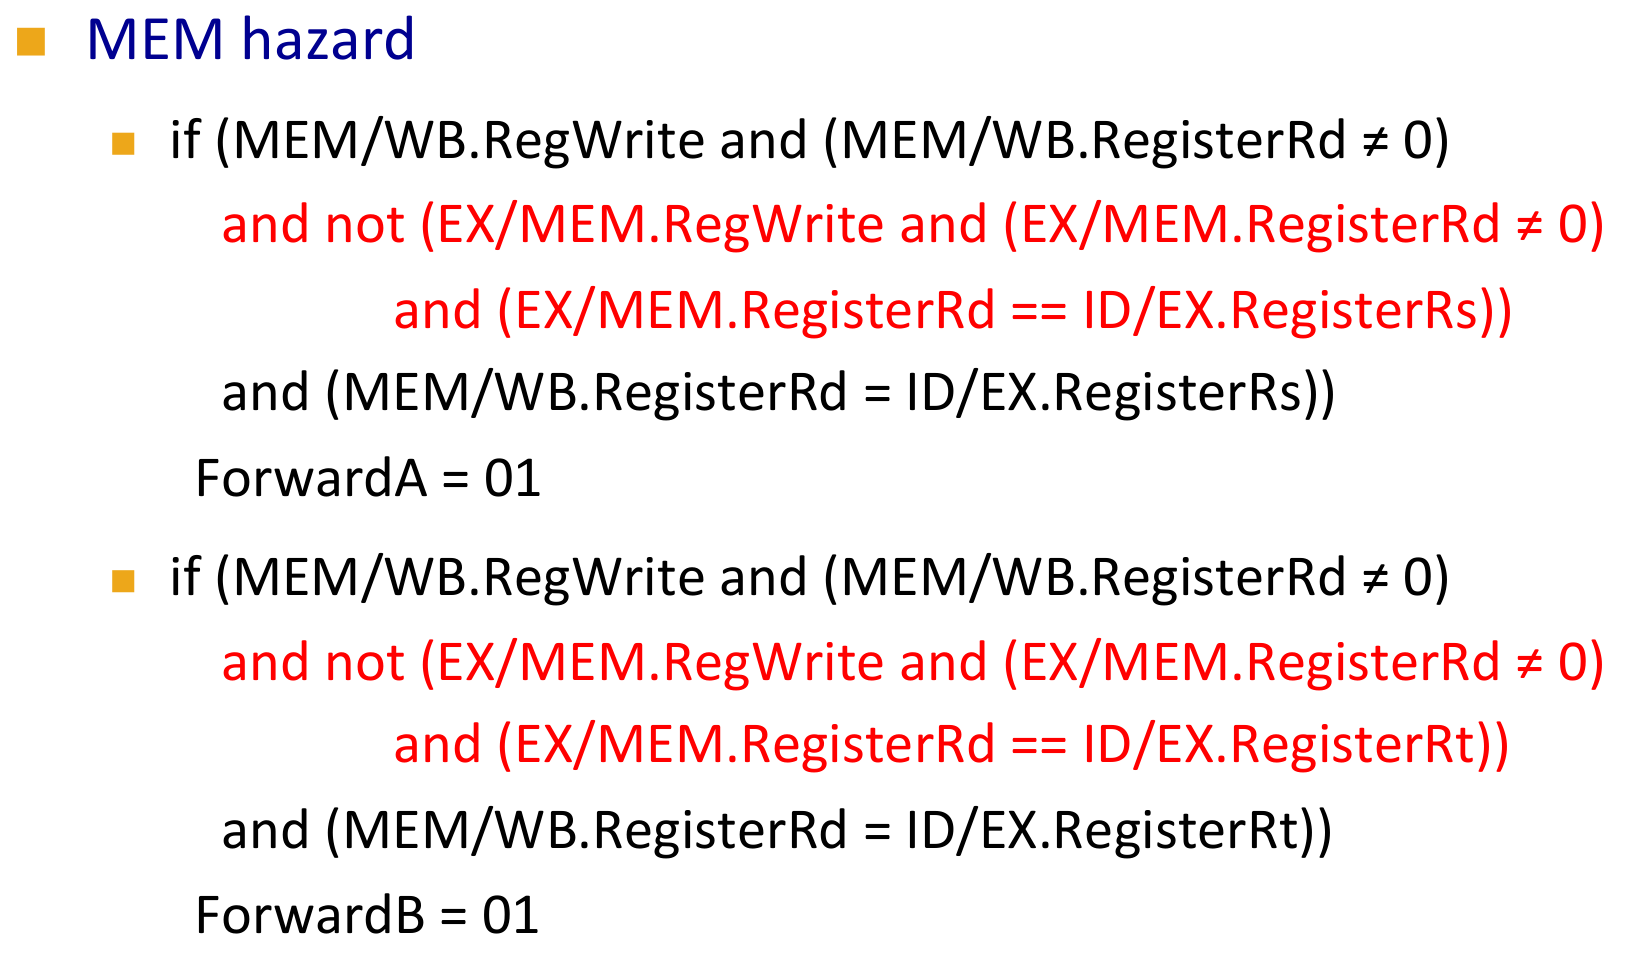
\includegraphics[width=\linewidth]{png/forwardingcontrol.png}

\subsection*{Control Hazards}
A control hazards is like a data hazard on the PC, we cannot fetch the next
instruction if we don't know the PC

Some solutions for control hazards are stalling on branches, predicting taken
or not taken. We need to flush the pipeline if we predict wrong, in a 5-sage
pipeline we only need to flush 1 instruction
